\documentclass[xcolor=dvipsnames,10pt]{beamer}
\usepackage{url}
\usepackage{multirow}
%% Define a new 'leo' style for the package that will use a smaller font.
\makeatletter
\def\url@leostyle{%
  \@ifundefined{selectfont}{\def\UrlFont{\sf}}{\def\UrlFont{\small\ttfamily}}}
\makeatother
%% Now actually use the newly defined style.
\urlstyle{leostyle}


  % ********** Styl prezentacji **********
  \mode<presentation>
  {
          \usetheme{Warsaw}
  }

  \author{Mahmoud Fatene \\ Frederic Durand \\ Valene Pellissier \\ Claire Yang}
  %\institute[...]{...}

  %\addtobeamertemplate{footline}{\insertframenumber}
  \subject{}
  \AtBeginSubsection[]
  {
          \begin{frame}<beamer>
                  \frametitle{Table of Contents}
                  \tableofcontents[currentsection,currentsubsection]
          \end{frame}
  }

  \title[Master Project]{Master Project}
  \subtitle{Water Sterilizer Optimization}

  \date{January 2008}

  %\AtBeginSubsection[]{
  %       \begin{frame}<beamer>
  %               \frametitle{Outline}
  %               \addtocounter{framenumber}{-1}
  %               \thispagestyle{empty}
  %               \tableofcontents[currentsection]
  %       \end{frame}
  %}
  \begin{document}


  \begin{frame}
          \titlepage
          \begin{figure}
          \raggedleft
          
\includegraphics[height=1cm, width=2cm]{./images/logoUJF.jpg}
          \hspace{65mm}
          \raggedright
          
\includegraphics[height=1.3cm, width=2cm]{./images/logoRCLux.jpg}
          \end{figure}
  \end{frame}

  \begin{frame}
          \frametitle{Table of contents}
          \tableofcontents
  \end{frame}

% Rclux ID
%{  \section{RC lux}

  \subsection{The beginning}

  \begin{frame}
          \frametitle{The beginning}
  \begin{itemize}[<+->]
  \item \textbf{Where? } Cosmology and subatomic physics laboratory in Grenoble
  \item \textbf{Who? } Pascal Sortais, plasma and ion sources specialist
	\begin{quotation}
	 I was, then, convinced that I could improve UV lamps technology. It was enough to adapt particle accelerators technologies to lower energies\footnote{Le journal la CNRS, \url{http://www2.cnrs.fr/presse/journal/2853.htm}}.
	\end{quotation} 
  \item \textbf{When? } 25 January 2006, RC Lux is created
	\end{itemize}
  \end{frame}

  \subsection{The steriliser}

  \begin{frame}
          \frametitle{The steriliser}
  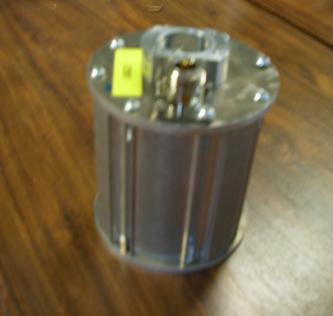
\includegraphics[height=4.5cm, width=4cm]{images/steriliser.jpg}
\hspace{0.5cm}
\begin{minipage}{0.5\linewidth}
 Award winner of most innovative technologies for environment
\end{minipage}
  

  \end{frame}
}

  \section{RC lux}

  \subsection{The beginning}

  \begin{frame}
          \frametitle{The beginning}
  \begin{itemize}[<+->]
  \item \textbf{Where? } Cosmology and subatomic physics laboratory in Grenoble
  \item \textbf{Who? } Pascal Sortais, plasma and ion sources specialist
	\begin{quotation}
	 I was, then, convinced that I could improve UV lamps technology. It was enough to adapt particle accelerators technologies to lower energies\footnote{Le journal la CNRS, \url{http://www2.cnrs.fr/presse/journal/2853.htm}}.
	\end{quotation} 
  \item \textbf{When? } 25 January 2006, RC Lux is created
	\end{itemize}
  \end{frame}

  \subsection{The steriliser}

  \begin{frame}
          \frametitle{The steriliser}
  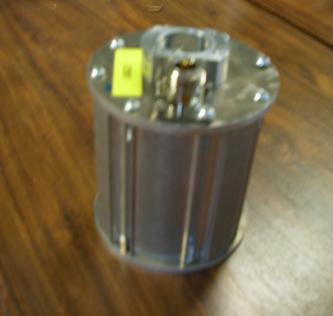
\includegraphics[height=4.5cm, width=4cm]{images/steriliser.jpg}
\hspace{0.5cm}
\begin{minipage}{0.5\linewidth}
 Award winner of most innovative technologies for environment
\end{minipage}
  

  \end{frame}
%%%%%%%%%%%%%%%%%%%%%%%%%Subject%%%%%%%%%%%%%%%%%%%%%%%%%%%%%%%%%%

  \section{Subject}

  \subsection{Definition}

  \begin{frame}
          \frametitle{Definition}
  \begin{itemize}[<+->]
  \item \textbf{Context:} To model water sterilization by UV radiation with this device :
          \begin{figure}
                  \raggedleft
                  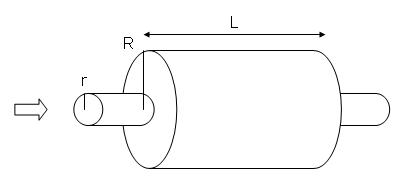
\includegraphics[width=5cm,height=2cm]{./images/sterilisateurh.jpg}
                  \hspace{3mm}
                  \raggedright
                  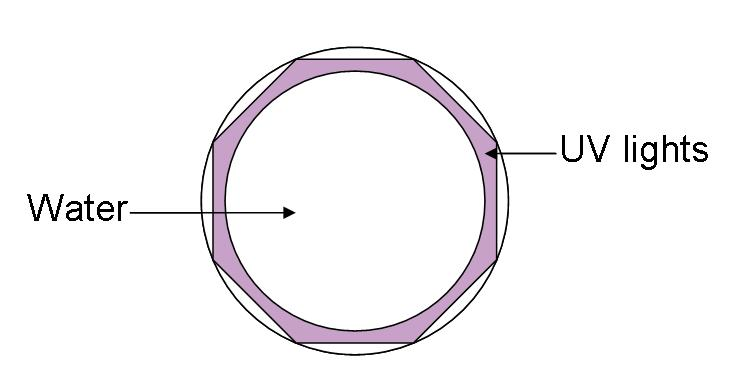
\includegraphics[width=4cm,height=2cm]{./images/coupeSterilisateur.jpg}
          \end{figure}
  \item \textbf{Goal:} To find the optimal radius $r$ and $R$ for which :
          \begin{itemize} 
                  \item[*] At the end of the pipe, the water is sterilized.
                  \item[*] The flow must be 2 or 4 $l.min^{-1}$.
                  \item[*] $R \in [7mm - 20mm]$ and $r \in [2mm - 6mm]$
          \end{itemize}
  \item \textbf{Expected Result:} To create a computer program to search these radius.
  \end{itemize}
  \end{frame}

  \subsection{Methodology}

  \begin{frame}
          \frametitle{Methodology}
  \begin{block}{Different concerned domains:}
  \begin{itemize}[<+->]
  \item Micro-Biology (bacteria's concentration)
  \item Fluid Mechanics
  \item Radiation
  \end{itemize}
  \end{block}
  \pause
  \invisible<1-2> {Our research approach: }
  \begin{block}{Simplified case $\Rightarrow$ real case:}
  \begin{itemize}[<+->]
  \item 0D mean velocity
  \item 1D mean velocity
  \item 2D axisymmetric with a Poiseuille's Profile
  \item 2D axisymmetric with simplified Navier-Stokes' equations
  \end{itemize}
  \end{block}
  \end{frame}


  \begin{frame}
          \frametitle{Methodology}
          \begin{figure}
                  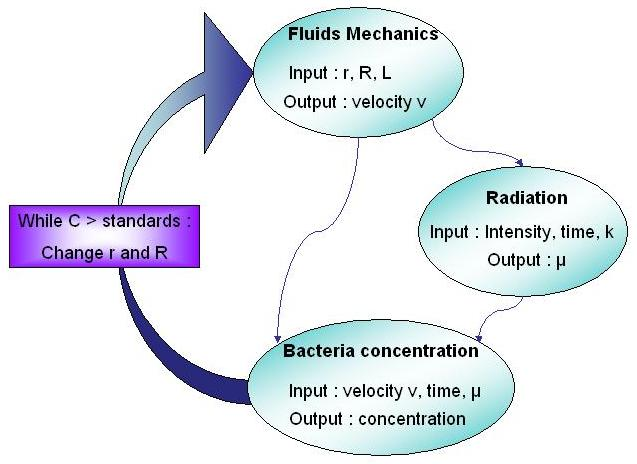
\includegraphics[width=9cm,height=7cm]{./images/methodology2.jpg}
          \end{figure}
  \end{frame}

  \subsection{Objectives}
  \begin{frame}
  \frametitle{Objectives}
  \underline{\textbf{\color{blue}First:}}\\
  \vspace{5mm}
  $\Rightarrow$ To complete the 0D model before mid-February.\\
  \vspace{4mm}
  $\Rightarrow$ To finish the 2D model and give representative results for $r$ and $R$ to obtain sterilised water.\\
  \vspace{8mm}
  \underline{\textbf{\color{blue}If miracle:}}\\
  \vspace{5mm}
  $\Rightarrow$ To do the same with the 3D model.\end{frame}



  %%%%%%%%%%%%%%%%%%%%%%%%%%%%%%%%%%%%%%%% MODELISATION %%%%%%%%%%%%%%%%%%%%%%%%%%%%%%%%%%%%%%%%%%%

  \section{Mathematical Models}

  \subsection{Fluids Mechanic}

  \begin{frame}
          \frametitle{General Case}
                  Incompressible fluids velocity are governed by Navier-Stokes equations. 
                  We look for the velocity $\vec{u}$ 
                  \begin{block}{The Navier-Stokes Equations}
                          \begin{equation}
                                  \left\{ \begin{array}{cl}
                                  \frac{\partial \vec{u}}{\partial t} + \vec{u}\cdot \nabla \vec{u} - u\Delta\vec{u} + \nabla p = f \\
                          \\
                                  div(\vec{u}) = 0
                                  \end{array}
                                  \right.
                          \end{equation}
                  \end{block}
                  where : 
          \begin{tabular}{ll}
                  $\vec{u}$: the fluid velocity\\
                  $p$: the pressure\\
          \end{tabular}
  \end{frame}

  %%%%%%%%%%%%%%%%%%%%%%%%%%%%%%%%%%%%%%%%%%%%%%%%%%%%%%%%%%%
  \begin{frame}
          \frametitle{0D Case}
                  {\footnotesize
                  \begin{itemize}
                          \item RC-Lux gives us: the pressure loss $\Delta p$ 
                          \item We look for: the velocity $v$ 
                  \end{itemize}
                  \begin{block}{The Darcy-Weisbach Equation (version 1)}
                          \begin{equation}
                                  h_l = f \cdot \frac{L}{D} \cdot \frac{v^2}{2g}
                          \end{equation}
                  \end{block}
                  where : 
          \begin{tabular}{ll}
                  $h_l$: the head loss due to friction\\
                  $f$: a Darcy friction factor\\
                  $L$: the length of the pipe and $D$: the diameter of the pipe\\
                  $g$: the gravitational constant
          \end{tabular}
                  \begin{block}{The Darcy-Weisbach Equation (version 2)}
                          Since $\Delta p = \rho g h_l$, where $\rho$ is the flow's density, we have :
                          \begin{equation}
                                  \Delta p = f \cdot \frac{L}{D} \cdot \frac{\rho v^2}{2}
                          \end{equation}
                  \end{block}
  }
  \end{frame}

  %%%%%%%%%%%%%%%%%%%%%%%%%%%%%%%%%%%%%%%%%%%%%%
  \begin{frame}
  \frametitle{0D Case}
          \begin{equation}
                  \Delta p = \left(\sum_{p=1}^3 f_p\frac{L_p}{D_p} + K_e + K_c\right)\cdot \frac{\rho v^2}{2}
          \end{equation}
  \begin{block}{Swamee-Jain Equation}
  \begin{equation}
          f_p = \frac{0.25}{[\log (\frac{\varepsilon}{3.7 D_p} + \frac{5.74\cdot \nu^{0.9}}{(v.D_p)^{0.9}})]^2}
  \end{equation}
  \end{block}
  And : \\
  \hspace{20mm}
  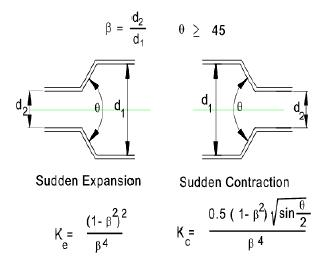
\includegraphics[height=30mm, width=5.5cm]{./images/fitting.JPG}
  \end{frame}



  %%%%%%%%%%%%%%%%%%%%%%%%%%%%%%%%%%%%%%%%%%%%%%%%%%%%% UV Radiation


  \subsection{UV Radiation}

  \begin{frame}
          \frametitle{General Case}
          \begin{block}{Single Stage Exponential Decay Equation}
                  \begin{equation}
                          S(t)=e^{-kIt}
                  \end{equation}
          \end{block}
          Where 
                  {\footnotesize 
                  \begin{tabular}{ll}
                          $S$: the surviving ratio of the initial population $\frac{c}{c_0}$\\
                          $t$: the exposure time\\
                          $I$: the UV radiation intensity\\
                          $k$: the sensitivity coefficient of the microorganisms to UV exposure.
                  \end{tabular}
                  } \\


          \begin{block}{Beer-Lambert Law}
                  \begin{equation}
                          I(x) = I_0\cdot e^{-\alpha x\rho}
                  \end{equation}
          \end{block}
          Where 
                  {\footnotesize 
                          \begin{tabular}{ll}
                          $I_0$ is the intensity of the incident light\\
                          $\alpha$, the absorption coefficient\\
                          $\rho$ the density of water.
                  \end{tabular}
                  }

  \end{frame}

  %%%%%%%%%%%%%%%%%%%%%%%%%%%%%%%%%%%%%%%%%%%%%% BACTERIA CONCENTRATION  %%%%%%%%%%%%%%%%%%%%%%%

  \subsection{Bacteria Concentration}

  \begin{frame}
          \frametitle{General Case}
          We are interested in solving this equation in order to know concentration at the end of the sterilizer. \\
          \begin{block}{Bacteria's Concentration Equation}
                  \begin{equation}
                          \frac{\partial{c}}{\partial{t}} + \underbrace{\vec{u}\cdot \nabla c}_{advection} + \underbrace{\mu\cdot c}_{reaction} = f
                  \end{equation}
          \end{block}
  Where,
          {\footnotesize
          \begin{tabular}{ll}
                  $c$: the bacteria concentration\\
                  $u$: the fluid velocity\\
                  $\mu$: a constant which represents the bacteria's destruction
          \end{tabular}
          }
  \end{frame}


  %%%%%%%%%%%%%%%%%%%%%%%%%%%%%%%%%%%%%%%%%%%% 0D
  \begin{frame}
          \frametitle{0D Case}
          In a first approximation:
          \begin{block}{Simplified Bacteria's Concentration Equation}
                  \begin{equation}
                          \left\{ \begin{array}{cl}
                          \frac{\partial{c}}{\partial{t}}= -\mu\cdot c\\
                          \\
                          c(t=0)=c_0
                          \end{array}
                          \right.
                  \end{equation}

           The solution of this problem is so: 
          \begin{equation}
                  c(t) = c_0\cdot e^{-\mu t}
          \end{equation}
          \end{block}

          Using the formula about radiation explained earlier, we obtain: 
          \begin{block}{The Concentration at time t:}
                  \begin{equation}
                          c(t) = c_0\cdot S(t) = c_0\cdot e^{-kIt}
                  \end{equation}
          \end{block}
  \end{frame}

%  %%%%%%%%%%%%%%%%%%%%%%%%%%%%%%%%%%%%%%%%%%%%Optimisation%%%%%%%%%%%%%%%%%%%%%%%%%%%%%%%%%%%%%%%%%%%
%{  \section{Optimisation}

  \subsection{Problem Formulation}
  \begin{frame}
  \frametitle{Problem Formulation}
  \begin{block}{Constrained optimisation problem}
  \begin{equation}
	\begin{cases}
  \mathop{Min}\limits _{(r,R)\in \mathcal{D}} \alpha C(r,R) + \beta Vol(r,R) \\
  C(r,R) \leq C_s\\
  2 \leq Q(r,R) \leq 4
	\end{cases}
  \end{equation}
  \end{block}

  \begin{itemize}
  \item $ \mathcal{D} = [2,6] \times [7,20]$
  \item  \emph{Vol} represents the volume of the device
  \item  $\alpha$ and $\beta$ weights on concentration and volume
  \item The dimension of the radius is the millimetre.\\
  \item We use $\Delta p = kQ^2$ to have the constraint on the flow.
  \end{itemize}
  \end{frame}

  \subsection{First Approximation}
  \begin{frame}
  \frametitle{First Approximation : $\beta = 0$}
  \begin{block}{Our optimisation problem}
$$ 
\begin{cases}
\mathop{\rm Min}\limits _{(r,R)} c(r,R) & = c_0 \exp{(-kI\frac{z}{U(r,R)})}\\
Q_1(r,R) & = 2-\pi r_{exit}^2U(r,R) \leq 0 \\
Q_2(r,R) & = \pi r_{exit}^2U(r,R) - 4 \leq 0
\end{cases}
$$
  \end{block}
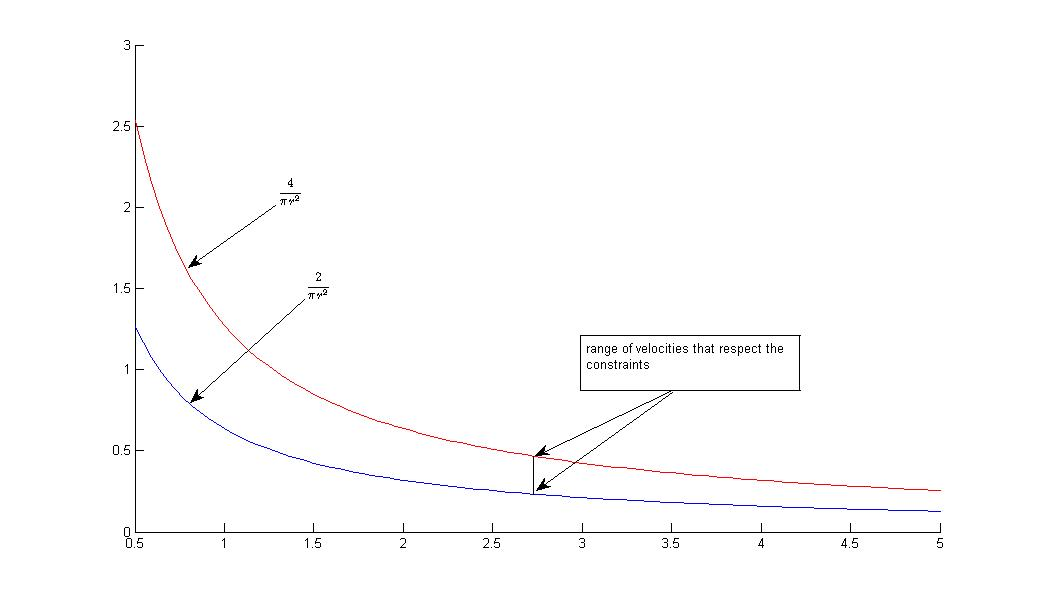
\includegraphics[height=4cm, width=5cm]{images/vrange.jpg}
\hspace{0.2cm}
\begin{minipage}{5cm}
$\frac{2}{\pi r^2} \leq U(r,R) \leq \frac{4}{\pi r^2}$
\end{minipage}
  \end{frame}

  \subsection{Second Approximation}
  \begin{frame}
  \frametitle{Second Approximation : $\beta = 0$ and $r=2mm$ $\Rightarrow \mathop{Min}\limits _{R\in [7,20]} C(R)$}
  \begin{block}{Formula}
  \begin{equation}
  \left(f_1(v)\frac{L_1+L_3}{2r} + f_2(v,R)\frac{L_2}{2R} + K_e + K_c\right)\cdot \frac{\rho v^2}{2} - \Delta p = 0
  \end{equation}
  \begin{equation}
  c(R) = c_0\cdot e^{-kI\frac{L_2}{v(R)}}
  \end{equation}
  \end{block}
  $1^{st}$ Step : $v(R)$ \hspace{40mm} $2^{nd}$ Step : $C(R)$
          \begin{figure}
          \raggedleft
          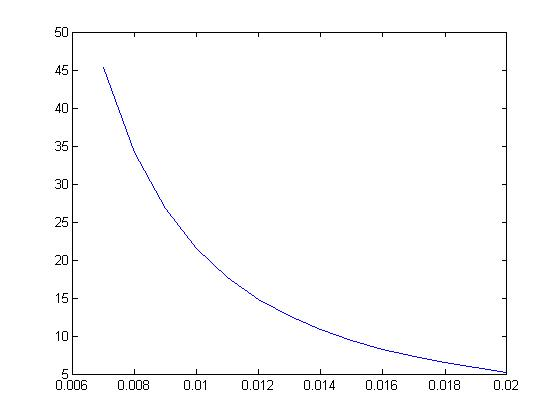
\includegraphics[height=3.1cm, width=5cm]{./images/graphVR.jpg}
          \hspace{5mm}
          \raggedright
          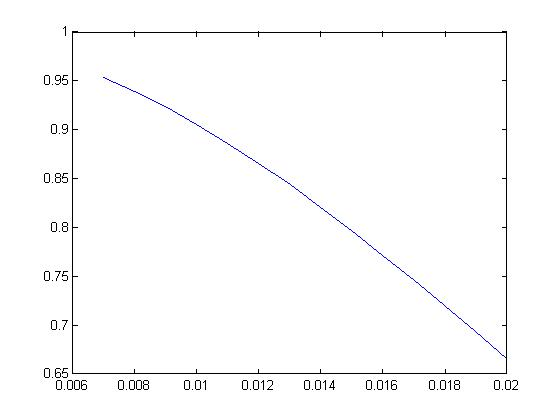
\includegraphics[height=3.1cm, width=5cm]{./images/graphCR.jpg}
          \end{figure}
  \end{frame}

  \subsection{In the Future}
  \begin{frame}
  \frametitle{In the Future}
  \begin{itemize}
  \item 0 Space Dimension :
          \begin{itemize} 
                  \item[*] To find the minimum bacteria concentration with $r$ and $R$.
                  \item[*] To optimize with the volume
          \end{itemize}
  \vspace{1cm}
  \item 1 Space Dimension
  \vspace{1cm}
  \item 2 Space Dimension

  \end{itemize}
  \end{frame}
}

  \section{Optimisation}

  \subsection{Problem Formulation}
  \begin{frame}
  \frametitle{Problem Formulation}
  \begin{block}{Constrained optimisation problem}
  \begin{equation}
	\begin{cases}
  \mathop{Min}\limits _{(r,R)\in \mathcal{D}} \alpha C(r,R) + \beta Vol(r,R) \\
  C(r,R) \leq C_s\\
  2 \leq Q(r,R) \leq 4
	\end{cases}
  \end{equation}
  \end{block}

  \begin{itemize}
  \item $ \mathcal{D} = [2,6] \times [7,20]$
  \item  \emph{Vol} represents the volume of the device
  \item  $\alpha$ and $\beta$ weights on concentration and volume
  \item The dimension of the radius is the millimetre.\\
  \item We use $\Delta p = kQ^2$ to have the constraint on the flow.
  \end{itemize}
  \end{frame}

  \subsection{First Approximation}
  \begin{frame}
  \frametitle{First Approximation : $\beta = 0$}
  \begin{block}{Our optimisation problem}
$$ 
\begin{cases}
\mathop{\rm Min}\limits _{(r,R)} c(r,R) & = c_0 \exp{(-kI\frac{z}{U(r,R)})} \textrm{ under the constraints} \\
Q_1(r,R) & = 2-\pi r_{exit}^2U(r,R) \leq 0 \\
Q_2(r,R) & = \pi r_{exit}^2U(r,R) - 4 \leq 0
\end{cases}
$$
  \end{block}
%\begin{tabular}{cc}
%\multirow{2}{*}{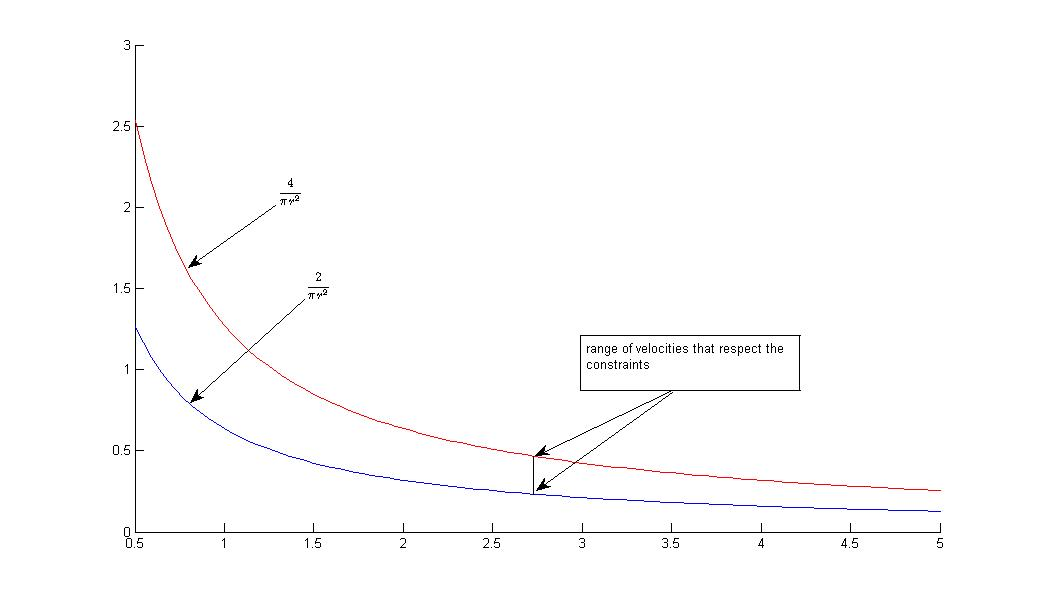
\includegraphics[height=4cm, width=5cm]{images/vrange.jpg}}&
%$\frac{2}{\pi r^2} \leq U(r,R) \leq \frac{4}{\pi r^2}$\\
%& 
%\end{tabular}

\hspace{0.2cm}
\begin{minipage}{5cm}
$\frac{2}{\pi r^2} \leq U(r,R) \leq \frac{4}{\pi r^2}$
\end{minipage}
  \end{frame}

  \subsection{Second Approximation}
  \begin{frame}
  \frametitle{Second Approximation : $\beta = 0$ and $r=2mm$ $\Rightarrow \mathop{Min}\limits _{R\in [7,20]} C(R)$}
  \begin{block}{Formula}
  \begin{equation}
  \left(f_1(v)\frac{L_1+L_3}{2r} + f_2(v,R)\frac{L_2}{2R} + K_e + K_c\right)\cdot \frac{\rho v^2}{2} - \Delta p = 0
  \end{equation}
  \begin{equation}
  c(R) = c_0\cdot e^{-kI\frac{L_2}{v(R)}}
  \end{equation}
  \end{block}
  $1^{st}$ Step : $v(R)$ \hspace{40mm} $2^{nd}$ Step : $C(R)$
          \begin{figure}
          \raggedleft
          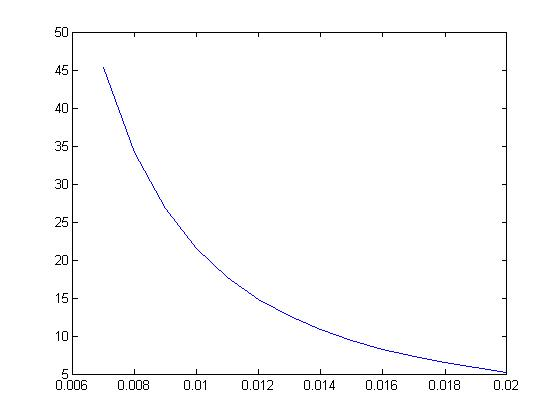
\includegraphics[height=3.1cm, width=5cm]{./images/graphVR.jpg}
          \hspace{5mm}
          \raggedright
          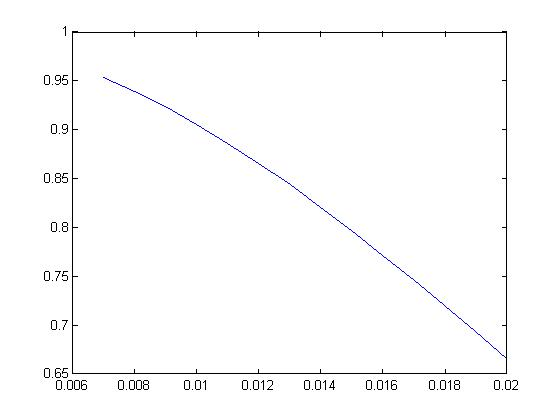
\includegraphics[height=3.1cm, width=5cm]{./images/graphCR.jpg}
          \end{figure}
  \end{frame}

  \subsection{In the Future}
  \begin{frame}
  \frametitle{In the Future}
  \begin{itemize}
  \item 0 Space Dimension :
          \begin{itemize} 
                  \item[*] To find the minimum bacteria concentration with $r$ and $R$.
                  \item[*] To optimize with the volume
          \end{itemize}
  \vspace{1cm}
  \item 1 Space Dimension
  \vspace{1cm}
  \item 2 Space Dimension

  \end{itemize}
  \end{frame}

%  \section{Optimization}
%
%  \subsection{Problem Formulation}
%  \begin{frame}
%  \frametitle{Problem Formulation}
%  \begin{block}{Formula}
%  \begin{equation}
%  \mathop{Min}\limits _{r\in [2,6];R\in [7,20];C<C_s} \alpha C(r,R) + \beta Vol(r,R) 
%  \end{equation}
%  \end{block}
%  \begin{itemize}
%  \item The dimension of the radius is the millimeter.\\
%  \item We use $\Delta p = kQ^2$ to have the constraint on the flow.
%  \end{itemize}
%  \end{frame}
%
%  \subsection{First Approximation}
%  \begin{frame}
%  \frametitle{First Approximation : $\beta = 0$ and $r=2mm$ $\Rightarrow \mathop{Min}\limits _{R\in [7,20]} C(R)$}
%  \begin{block}{Formula}
%  \begin{equation}
%  \left(f_1(v)\frac{L_1+L_3}{2r} + f_2(v,R)\frac{L_2}{2R} + K_e + K_c\right)\cdot \frac{\rho v^2}{2} - \Delta p = 0
%  \end{equation}
%  \begin{equation}
%  c(R) = c_0\cdot e^{-kI\frac{L_2}{v(R)}}
%  \end{equation}
%  \end{block}
%  $1^{st}$ Step : $v(R)$ \hspace{40mm} $2^{nd}$ Step : $C(R)$
%          \begin{figure}
%          \raggedleft
%          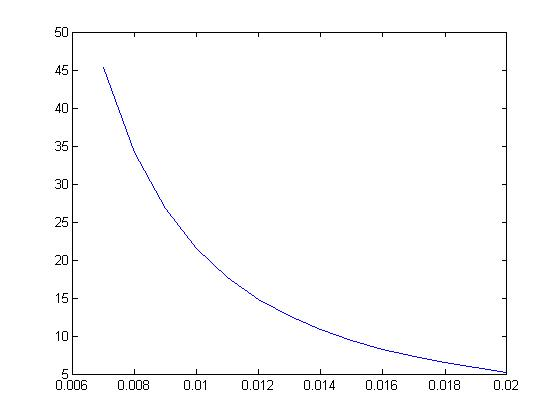
\includegraphics[height=3.1cm, width=5cm]{./images/graphVR.jpg}
%          \hspace{5mm}
%          \raggedright
%          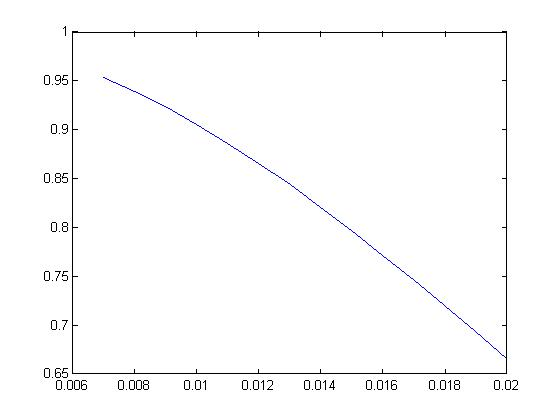
\includegraphics[height=3.1cm, width=5cm]{./images/graphCR.jpg}
%          \end{figure}
%  \end{frame}
%
%  \subsection{In the Future}
%  \begin{frame}
%  \frametitle{In the Future}
%  \begin{itemize}
%  \item 0 Space Dimension :
%          \begin{itemize} 
%                  \item[*] To find the minimum bacteria concentration with $r$ and $R$.
%                  \item[*] To optimize with the volume
%          \end{itemize}
%  \vspace{1cm}
%  \item 1 Space Dimension
%  \vspace{1cm}
%  \item 2 Space Dimension
%
%  \end{itemize}
%  \end{frame}

  %%%%%%%%%%%%%%%%%%%%%%%%%%%%%Conclusion%%%%%%%%%%%%%%%%%%%%%%%%%%%%%%%%%%%%

  \section{Conclusion}

  \begin{frame}
          \frametitle{Conclusion}
  \underline{\textbf{\color{blue}Difficulties:}}\\
   \begin{itemize}
    \item Delay in our schedule.
    \item More complex than we expected.
    \item Almost no communication with the RC-Lux company.
    \end{itemize}

  \underline{\textbf{\color{blue}Positive Points:}}\\ 
   \begin{itemize}
    \item Very interesting and concrete subject with different scientific domains.
    \item Learning of many things.
    \item Participation to an industrial project.
   \end{itemize}
  \end{frame}

  \begin{frame}
  \vspace{8mm}
  \hspace{4mm}
  \huge{\textbf{\color{blue}Thank you for your attention}}
  \end{frame}

  \end{document}
